%\begin{frame}
    %\frametitle{Planificación}

      %  \begin{block}{Propuesta del PFC}
     %       A finales de Mayo del 2010 se comenzó a plantear que se podía realizar como proyecto fin de carrera. 
    %        Tuvo lugar las reuniones con el tutor, con el fin de obtener distintas ideas. Finalmente entre todas las ideas
   %         propuestas se decidió realizar este proyecto.
  %      \end{block}
 %       
%\end{frame}

\begin{frame}
    \frametitle{Planificación}

        \begin{block}{Tiempo de desarrollo}
            De septiembre de 2010 a septiembre de 2011.
        \end{block}
    
        \begin{block}{Fases}
        Durante el periodo de desarrollo tuvieron lugar las distintas fases:
            \begin{itemize}
                \item \textbf{Fase de análisis}: indentificación de las necesidades del software
                \item \textbf{Fase de diseño}: diseño de todo el sistema
                \item \textbf{Fase de aprendizaje}: familiarización con el lenguaje python y la biblioteca pygame
                \item \textbf{Fase de desarrollo}: implementación de todo los obtenido en la fase de diseño. Fase más larga
                \item \textbf{Pruebas y correcciones}: pruebas necesarias para comprobar el correcto funcionamiento. En paralelo a
                la fase de desarrollo
                \item \textbf{Redacción de la memoria}: realización de la memoria final
            \end{itemize}
        \end{block}

\end{frame}

\begin{frame}
    \frametitle{Diagrama de Gantt I}

        \begin{center}
                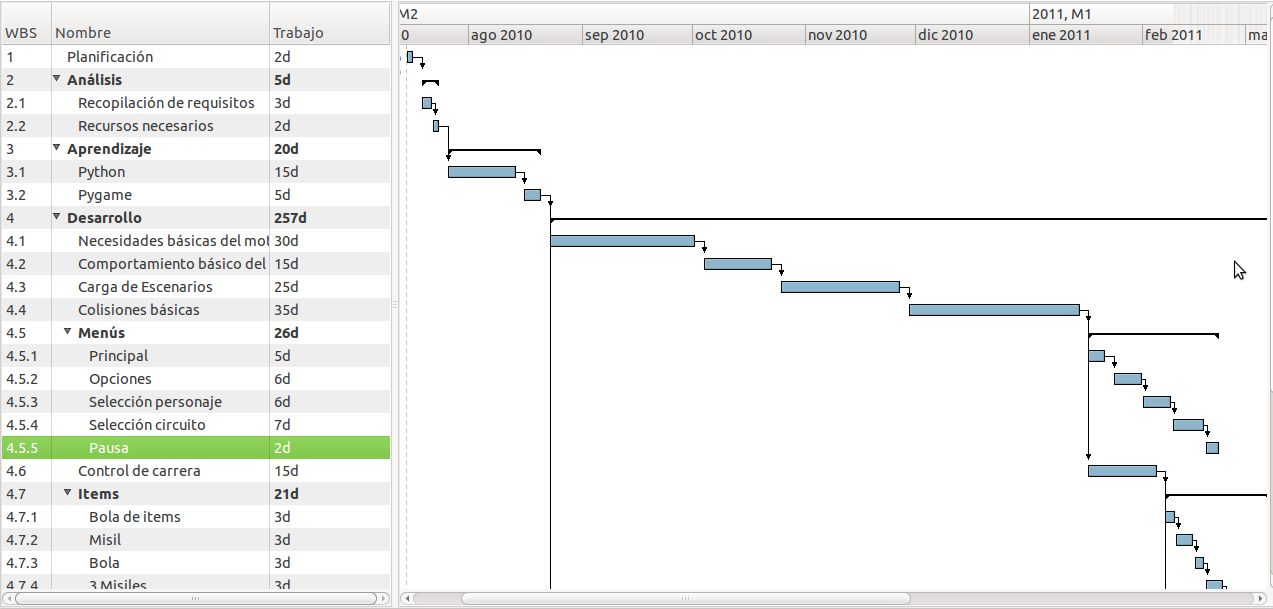
\includegraphics[scale=0.25]{imagenes/gant1.png}
        \end{center}
\end{frame}

\begin{frame}
    \frametitle{Diagrama de Gantt II}
        \begin{center}
                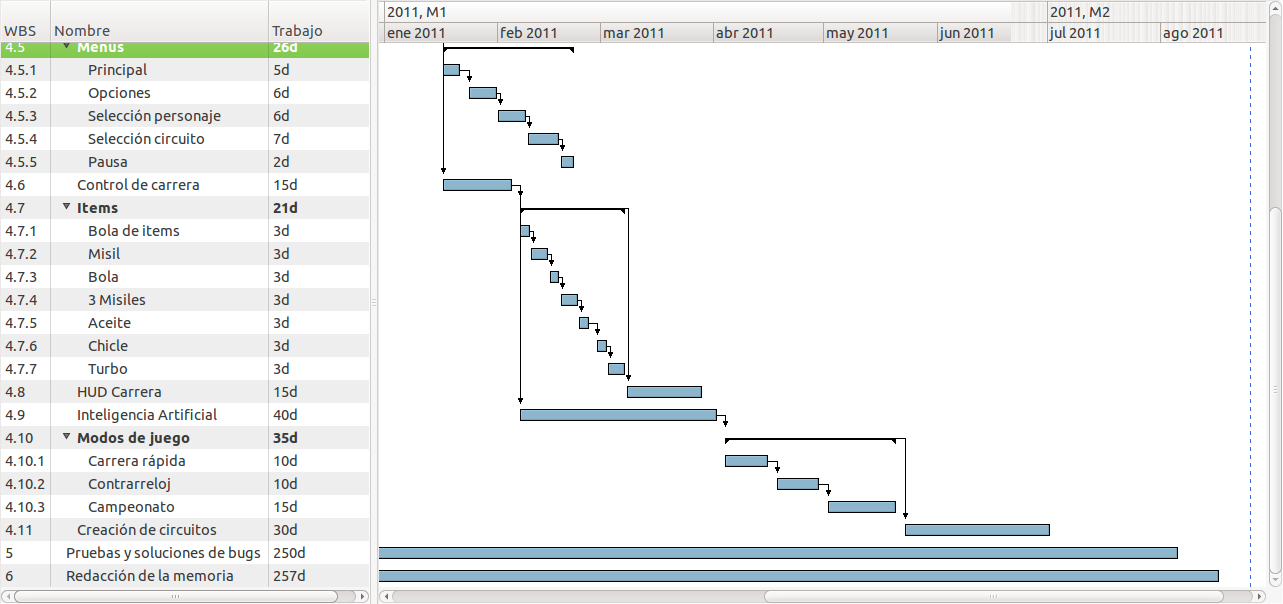
\includegraphics[scale=0.25]{imagenes/gant2.png}
        \end{center}
\end{frame}
